% ========================================
% CAPÍTULO 3: METODOLOGÍA, DATOS Y HOJA DE RUTA  (criterio 3)
% ========================================

\chapter{METODOLOGÍA, DATOS Y HOJA DE RUTA}
\label{ch:metodologia}

\section{Metodología: protocolo experimental en cinco fases}
\label{sec:fases}

Se adapta CRISP-DM a la construcción de un instrumento de medición: siguiendo la lógica de \emph{design science}, se construye un artefacto y se evalúa contra una verdad conocida \parencite{hevner2004}. El flujo anterior, de 19 etapas, se reemplazó por un protocolo lineal de cinco fases deterministas (Tabla~\ref{tab:etapas}). Cada fase tiene un propósito ligado a un objetivo específico, un script que la ejecuta y un artefacto que la deja verificable; todas se reproducen con \arch{python run_all.py}.

\begin{table}[!htbp]
\centering
\caption{Protocolo en cinco fases: propósito, implementación y evidencia.}
\label{tab:etapas}
\begingroup\scriptsize\singlespacing
\begin{tabular}{@{}p{2.7cm} p{2.0cm} p{3.9cm} p{3.4cm} p{2.3cm} p{0.8cm}@{}}
\toprule
Fase & CRISP-DM & Propósito & Script & Artefacto & OE \\
\midrule
0. Datos & Comprensión y preparación & Cargar y caracterizar 6 datasets; ruido y faltantes reproducibles & \arch{sklearn_loader.py}; \arch{eda_datasets.py} & \arch{eda_datasets.csv} & OE3 \\
1. Banco de control & Preparación & Escribir 96 pares con y sin fuga (oráculo programático) & \arch{generate_controlled_pairs.py} & 192 scripts & OE1 \\
2. Auditoría & Modelado del instrumento & Auditar cada script con AST y con verificación en ejecución & \arch{03_auditor/}; \arch{run_benchmark.py} & \arch{auditor_per_script.csv} & OE2 \\
3. Eficacia del auditor & Evaluación & Comparar veredictos con la verdad conocida y con la línea base & \arch{run_benchmark.py}; \arch{independent_evaluation.py} & Tablas \ref{tab:banco}--\ref{tab:base} & OE2 \\
4. Sesgo de optimismo & Evaluación & Calcular \DOpt{} por par, pruebas por familia y control positivo & \arch{statistical_analysis.py}; \arch{noise_sensitivity.py} & Tablas \ref{tab:dopt}--\ref{tab:tests} & OE3 \\
5. Empaquetado & Despliegue & Publicar el auditor como dos Skills y una plataforma web & \arch{05_skills/}; \arch{06_web_app/} & Cap.~\ref{ch:aplicabilidad} & OE4 \\
\bottomrule
\end{tabular}
\endgroup
\end{table}
\donde{OE: objetivo específico. La fase 0 prepara los insumos de las cinco fases experimentales.}

\section{Datos: origen, obtención y caracterización}
\label{sec:datos}

Se usan seis conjuntos nativos de scikit-learn (Tabla~\ref{tab:datasets}): tres de clasificación (\texttt{breast\_cancer}, \texttt{wine}, \texttt{digits}) y tres de regresión (\texttt{diabetes}, \texttt{california\_housing}, \texttt{make\_friedman1}). Son públicos, no contienen datos personales y se cargan sin copiarlos al repositorio; solo \texttt{california\_housing} se descarga la primera vez. La Figura~\ref{fig:eda} resume la dispersión de escalas y el balance de clases.

\begin{table}[!htbp]
\centering
\caption{Caracterización de los datasets.}
\label{tab:datasets}
\begingroup\footnotesize\singlespacing
\begin{tabular}{@{}l l l r r r r r@{}}
\toprule
ID & Dataset & Tarea & $N$ & Variables & Razón de escalas & Asimetría media & Clase minoritaria \\
\midrule
D1 & breast\_cancer & Clasif. (2) & 569 & 30 & 215.171 & 1,74 & 37,3\,\% \\
D2 & wine & Clasif. (3) & 178 & 13 & 2.530 & 0,43 & 27,0\,\% \\
D3 & digits & Clasif. (10) & 1.797 & 64 & 277 & 4,89 & 9,7\,\% \\
D4 & diabetes & Regresión & 442 & 10 & 1,0 & 0,41 & --- \\
D5 & california\_housing & Regresión & 3.000$^{*}$ & 8 & 1.398 & 10,00 & --- \\
D6 & friedman1 & Regresión & 1.000 & 50 & 1,1 & 0,04 & --- \\
\bottomrule
\end{tabular}
\endgroup
\end{table}
\nota{Razón de escalas: desviación estándar máxima sobre mínima entre variables. $^{*}$Submuestra determinista de 3.000 filas de 20.640 (desviación B1, sección~\ref{sec:desviaciones}). \texttt{digits} tiene 3 columnas constantes.}

\textbf{Calidad más allá de los faltantes.} Ningún dataset base tiene filas duplicadas. La proporción de celdas atípicas ($|z|>3$ por columna) es baja: 1,24\,\% en \texttt{breast\_cancer}, 0,48\,\% en \texttt{wine}, 0,67\,\% en \texttt{digits}, 0,34\,\% en \texttt{diabetes}, 0,59\,\% en \texttt{california\_housing} y 0\,\% en \texttt{friedman1} (\arch{eda_datasets.csv}). Son datos limpios por diseño, y por eso los faltantes se simulan.

\begin{figure}[!htbp]
\centering
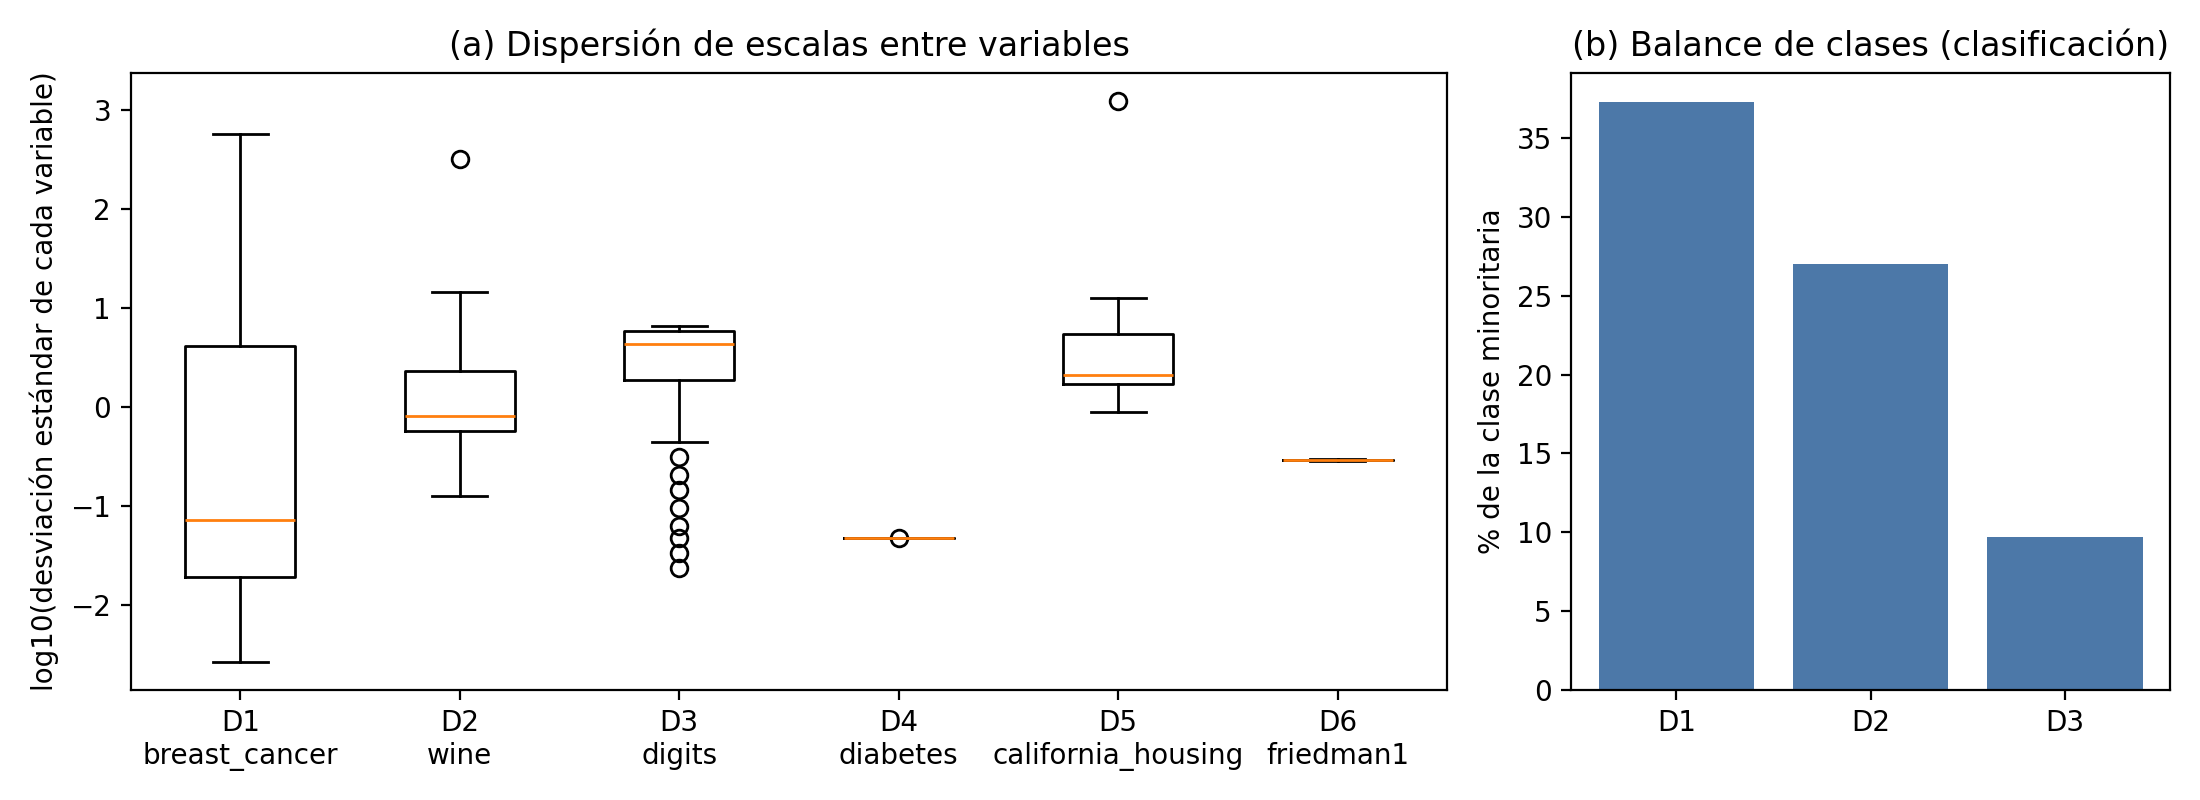
\includegraphics[width=0.82\textwidth]{fig_eda_datasets.png}
\caption{(a) Dispersión de escalas entre variables, en $\log_{10}$ de la desviación estándar. (b) Porcentaje de la clase minoritaria en los datasets de clasificación.}
\label{fig:eda}
\end{figure}

\textbf{Preparación trazable.} (i) \emph{Variante «completo»}: sin faltantes. (ii) \emph{Variante «con\_faltantes»}: se borra el 10\,\% de las celdas con semilla fija (media observada entre 9,8 y 10,1\,\%). (iii) A D1--D5 se les agregan 50 columnas de ruido gaussiano, porque la fuga por selección solo se manifiesta si hay variables inútiles entre las cuales elegir; D6 ya trae 45. Todo usa la semilla 42, y dos ejecuciones producen datos idénticos (verificado en las pruebas automáticas).

\textbf{Representatividad y limitaciones.} Son datasets clásicos, limpios, pequeños y tabulares; no representan datos reales ruidosos, de gran escala ni con estructura temporal o jerárquica, y los LLM probablemente los vieron durante su entrenamiento. Por la dispersión de escalas (Figura~\ref{fig:eda}a), el escalado debería afectar sobre todo a los modelos sensibles a la escala; por la asimetría de D5 (10,0) se esperan valores atípicos que desestabilicen a la red neuronal, y así ocurrió (sección~\ref{sec:desviaciones}). Con ROC-AUC cercana a 1 en D1--D3 hay un efecto techo que limita cuánto optimismo puede observarse en clasificación.

\section{Diseño experimental y arquitectura por fase}
\label{sec:diseno}
\label{sec:arquitectura}

Para cada combinación de 6 datasets $\times$ 4 familias $\times$ 4 tipos de fuga, un generador escribe un script con fuga (\texttt{leaky}) y otro idéntico sin ella (\texttt{clean}): \textbf{96 pares, 192 scripts}. Los modelos son \texttt{RandomForest}, \texttt{HistGradientBoosting}, \texttt{LogisticRegression} o \texttt{Ridge}, y \texttt{MLPClassifier} o \texttt{MLPRegressor}, todos de scikit-learn \parencite{pedregosa2011}. Como la verdad se conoce por construcción, no se necesitan anotadores.

Cada script se audita con \textbf{dos mecanismos independientes}. El primero analiza el árbol sintáctico (\texttt{ast}) con tres reglas: \emph{R-Split} (ajuste antes de \texttt{train\_test\_split}), \emph{R-CV} (ajuste fuera de un \texttt{Pipeline} cuyo resultado entra a la validación cruzada) y \emph{R-Test} (ajuste con una variable que parece de prueba). El segundo es un verificador en ejecución que cuenta con cuántas filas se ajusta cada transformador y declara fuga si coincide con el total del dataset. El detector híbrido declara fuga si cualquiera de los dos la ve.

Para evitar el sesgo de autopreferencia, el protocolo separa a los sujetos de estudio del sistema de medición (Tabla~\ref{tab:arquitectura}): ningún LLM participa en la auditoría ni en el cálculo de las métricas.

\begin{table}[!htbp]
\centering
\caption{Arquitectura por fase: quién genera y quién audita.}
\label{tab:arquitectura}
\begingroup\scriptsize\singlespacing
\begin{tabular}{@{}p{3.0cm} p{4.2cm} p{5.6cm} p{1.6cm}@{}}
\toprule
Componente & Rol & Implementación & ¿Usa LLM? \\
\midrule
Conjunto A (generador) & Sujetos de estudio: pipelines escritos por LLM & Mismo \emph{prompt} para todos; versión exacta y fecha registradas (Capstone~II) & Sí \\
Conjunto B (banco de control) & Verdad conocida por construcción & \arch{generate_controlled_pairs.py}: 96 pares con y sin fuga & No \\
Conjunto manual & Control de la circularidad & 13 scripts escritos a mano con estilos que el generador no produce & No \\
Motor auditor & Instrumento de medición & AST (tres reglas) y verificación en ejecución; salida idéntica en cada corrida & No \\
\bottomrule
\end{tabular}
\endgroup
\end{table}

\section{Hoja de ruta actualizada y desviaciones}
\label{sec:desviaciones}

\begin{table}[!htbp]
\centering
\caption{Hoja de ruta con hitos y entregables (estado a octubre de 2026).}
\label{tab:plan}
\begingroup\scriptsize\singlespacing
\begin{tabular}{@{}p{2.4cm} p{6.6cm} p{4.6cm} p{1.4cm}@{}}
\toprule
Periodo & Actividad & Hito o entregable verificable & Estado \\
\midrule
Capstone I & Reformulación del problema y la métrica; datasets; banco de 96 pares; auditor AST y de ejecución; refactorizador; \DOpt; Skills y plataforma web (prototipo) & Repositorio público reproducible con un comando; este informe & Hecho \\
Capstone II, sem. 1--4 & Generar pipelines con 6--8 LLM reales (24 tareas por modelo) y auditarlos; ejecutarlos en un contenedor aislado & Conjunto A versionado; tasa de fuga por modelo con IC95\,\% & Pendiente \\
Capstone II, sem. 5--8 & Mejorar el auditor (alias de importación, funciones auxiliares, \texttt{ColumnTransformer}); ampliar la evaluación independiente de 13 a $\geq 60$ scripts & Auditor v2 con recall independiente $\geq 0{,}80$ (umbral fijado antes de evaluar) & Pendiente \\
Capstone II, sem. 9--12 & Datasets con señal débil; \DOpt{} por tramo de señal/ruido; piloto de uso con 3--5 personas & Tabla de \DOpt{} condicionada; informe del piloto & Pendiente \\
Capstone II, sem. 13--16 & Redacción final y defensa & Documento final y presentación & Pendiente \\
\bottomrule
\end{tabular}
\endgroup
\end{table}

\textbf{Desviaciones respecto del plan original} (justificación completa en \arch{07_report/decision_log.md}):
\begin{itemize}
  \item \textbf{B1.} \texttt{california\_housing} se submuestrea a 3.000 filas: \texttt{KNNImputer} crece con $n^2$ y el banco de 192 scripts no sería ejecutable en un portátil.
  \item \textbf{B2.} El sobremuestreo (SMOTE) no se mide, porque no pertenece a scikit-learn; el cuarto tipo es «combinada».
  \item \textbf{C1.} En la primera corrida, los modelos lineal y MLP sin escalar daban diferencias negativas por inestabilidad numérica (hasta $-0{,}155$ en \texttt{wine}); se añadió un escalador interno idéntico en ambas versiones (corrida descartada en \arch{results/run1_discarded/}).
  \item \textbf{C2.} Un \texttt{MLPRegressor} divergió en un pliegue ($R^2=-21$ en \texttt{california\_housing}; promedio $-3{,}86$). Se definió, \textbf{después de ver el problema}, que un par es degenerado si algún pliegue tiene $R^2<-1$; se excluyó 1 par de 96 y se lista aparte.
\end{itemize}
